\chapter{Preliminaries}
\label{sec:theory}
In this chapter, we provide some background knowledge that will be required for understanding future parts of the thesis.

\section{Hash Functions}
A bit-oriented hash function~\cite{preneel1994cryptographic} is a mathematical function $H : \{0,1\}^* \rightarrow \{0,1\}^n$ with $n\geq1$ which takes an input (or 'message') of variable length and computes a fixed length output.

A hash function generally starts by dividing the input data into fixed size blocks. This is necessary because hash functions operate on data with a fixed length, and the input could be of any length. This padding process varies depending on the details of the hash function.

\subsection*{Properties}
To be an effective cryptographic tool, the hash function needs to posses the following properties~\cite{preneel1993analysis}:
\begin{itemize}
    \item \textbf{One way function (pre-image resistance):} It should be computationally difficult to reverse a hash funtion.
    \item \textbf{Target collision resistance (Second pre-image resistance):} Given an input and its hash, it should be computationally difficult to find a different input with the same hash.
    \item \textbf{Collision resistance:} It should be computationally difficult to find two different inputs of any arbitrary length that result in the same hash value.
    \item \textbf{Deterministic:} The same input will always produce the same output.
    \item \textbf{Efficiency:} The hash function must compute values quickly to ensure practical usability.
\end{itemize}

\subsection{Block ciphers}
Block ciphers~\cite{knudsen1999block} are symmetric key cryptographic alogrithms that operates on fixed length groups of bits, called blocks. The alogrithm accepts an input block of size $n$ bits and a key of size $k$ bits, and produce an $n$ bits output block. They are designed to be reversible, meaning the ciphertext can be transformed back into the plaintext using the same key.
\begin{equation}
    E:\{0,1\}^k\times\{0,1\}^n\rightarrow\{0,1\}^n.
\end{equation}

Block ciphers usually use multiple rounds of operations, including permutations and substitutions, until inverting the function becomes hard. They can be used to construct hash functions.

\textit{Feistel networks}, \textit{Substitution-Permutation Networks} (SPNs), \textit{Horst} schemes and \textit{open Flyestel} components are fundamental structures used to design block ciphers.

\subsubsection*{Feistel Networks}
A Feistel network~\cite{10.1007/BFb0034838, feistel1973cryptography} is a structure used to construct block ciphers. The input block $X$ is divided into two parts $X_1\text{ and }X_2$. One round of a Feistel network is defined as follows:
\begin{flalign*}
    Y_1=X_1\oplus F(X_2,K) \\
    Y_2=X_2 \\
    Y_1'=Y_2 \\
    Y_2'=Y_1,
\end{flalign*}
where $K$ is the round key, $F$ is the round function and $(Y_1',Y_2')$ is the data output of the round taken as input to the next round.

The Feistel network provides difussion of the input blocks. After two rounds of the network the dissufion is complete, that is, both output blocks depend on both input blocks.

\subsubsection*{Substitution-permutation network}
Substitution-permutation network (SPN)~\cite{feistel1973cryptography, shannon1949communication} is used to generate block ciphers. It is a repeated series of mathematical operations.

SPN takes an input block of the plaintext and a key as the input, and applies substitution (S-box) and Permutation (P-box) to each round.\\
An \textbf{S-box} substitues each byte of the input block with another byte. This layer of the SPN introduces non-linearity.\\
A \textbf{P-box} is a permutation of every bit: the bits of the S-box output are permuted, and then are passed to the S-box of the next round.

Thus, in SPN consists on three primary operations in each round: addition of a round key, substitution and permutation.

\subsubsection*{Horst scheme}
\label{sec:horst}
Horst is another structure that can be used to design block ciphers, it is defined in~\cite{grassi2022horst} and used in the Griffin hash function design. Let $t\geq2$. For each $i\in{1,2,\dots,t-1}$, let $G_i:\mathbb{F}_q^i\rightarrow\mathbb{F}_q\backslash\{0\}$ and $\mathbb{F}_i:\mathbb{F}_q^i\rightarrow\mathbb{F}_q$. Horst is defined over $\mathbb{F}_q^t$ as $x=(x_0,\dots,x_{t-1})\mapsto y=(y_0,\dots,y_{t-1})$, where
\begin{equation*}
    y_i:=\begin{cases}
        x_{i+1}\cdot G_{i+1}(x_0,x_1,\dots,x_i)+F_{i+1}(x_0,x_1,\dots,x_i) & \text{if } i\in{0,1,\dots,t-2}, \\
        x_0 & \text{otherwise } (i=t-1).
    \end{cases}
\end{equation*}

The final circular shift is crucial for achieving full diffusion (as in the case of any Feistel scheme), but it can be replaced with a different linear diffusion.

\subsubsection*{Open Flyestel structure}
\label{sec:flyestel}
The \textit{open Flyestel} structure is a non-linear component presented and used in the design of Anemoi~\cite{bouvier2023new}.

Let $Q_\gamma:\mathbb{F}q\rightarrow\mathbb{F}_q$ and $Q_\delta:\mathbb{F}_q\rightarrow\mathbb{F}_q$ be two quadratic functions, and let $E:\mathbb{F}_q\rightarrow\mathbb{F}_q$ be a permutation. Then, the \textit{Flyestel} is a pair of functions relying on $Q_\gamma, Q_\delta$ and $E$. The \textit{open Flyestel} is the permutation of $(\mathbb{F}_q)^2$ obtained using a 3-round Feistel network with $Q_\gamma, E^{-1}$, and $Q_\delta$ as round functions. It is defined as $\mathcal{H}(x,y)=(u,v)$.
\begin{equation}
    \begin{cases}
        x\leftarrow x-Q_\gamma(y), \\
        y\leftarrow y-E^{-1}(x), \\
        x\leftarrow x+Q_\delta(y), \\
        u\leftarrow x,v\leftarrow y.
    \end{cases}
\end{equation}

\section{Sponge structure}
\label{sec:sponge-construction}
The sponge construction will be used in the different hash functions that are implemented on this thesis.

\subsection*{Overview}
The sponge construction maps an input of arbitrary length to an arbitrary length output. So the input don't have any restriction of his length, and the output length is not determined by the input~\cite{guido2011cryptographic}.

The sponge construction is built over an internal permutation, $\mathcal{P}$, that operates on the $\mathbb{F}_q^{r+c}$. This permutation works on a state with a length of $t$ called the width, where $t=r+c$, $r$ is the rate (outer part of the state) and $c$ the capacity (inner part of the state). The digest consists of $h$ elements.

A sponge can be used to obtain hash function: you use the sponge to absorb the input data, and then squeeze out just enough to form a hash. This approach enables hash functions to handle inputs of varying lengths while producing fixed-length outputs.
Figure~\ref{fig:sponge-hash} explains the principle of the Sponge construction.

First, the state is initialized to zero, and the following operations are made to the input message $m$:
\begin{enumerate}
    \item \textbf{Padding:} The padding rule of the sponge works as follows: when the length of the input message is not a multiple of the rate of the sponge, we append 1$\in\mathbb{F}_q$ to the input followed by enough zeros to make it a multiple of $r$, and split the message into blocks of size $r$, called chunks.
    \item \textbf{Absorbing:} When the input is divided into blocks of size $r$ (chunks), they are absorbed into the state of the sponge construction. Each one of these blocks is added to the outer part of the state using vector addition in $\mathbb{F}^r$ (where $\mathbb{F}$ is a finite field), and then the permutation is applied to it. This process is repeated for each block.
    \item \textbf{Squeezing:} In this phase the output is produced by extracting min$\left(h,r\right)$ elements from the outer part of the state $r$. If $r<h$, we apply the permutation $\mathcal{P}$ and extract the $r$ elements, this process is repeated until we reach the desired output length $h$.
\end{enumerate}
The length of the output, $h$, can be arbitrarily chosen.

\begin{figure}[htbp]
    \centering
    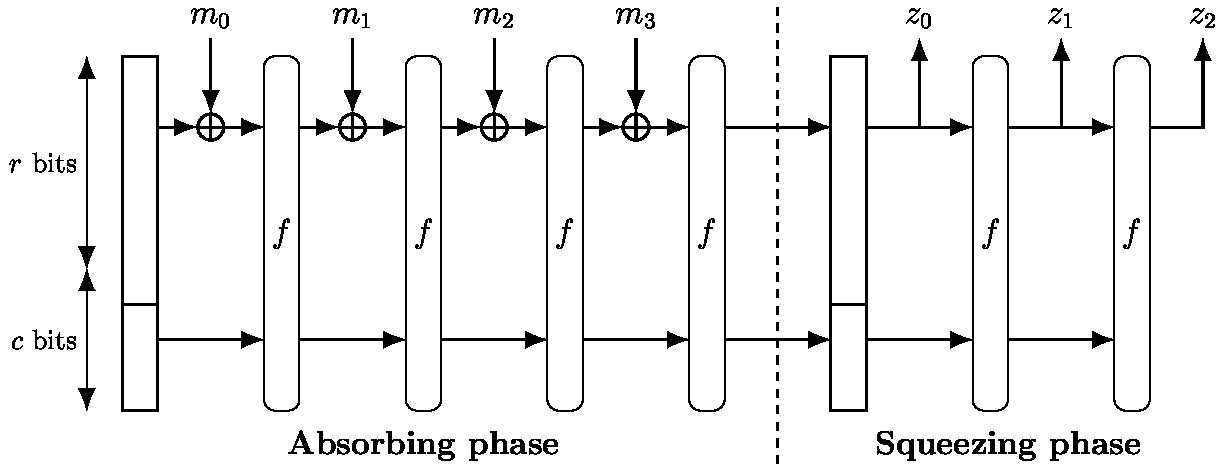
\includegraphics[width=\textwidth]{graphics/sponge.png}
    \caption{Sponge construction with 4 input chunks and a permutation $f$.}
    \label{fig:sponge-hash}
\end{figure}

\subsection{Cryptographic permutation}
A cryptographic permutation is a function that maps an input to an unique output of the same length. The function is designed to be bijective, every input has a unique output. It consists in a sequence of operations iterated over $R$ rounds. This sequence of operations are called the round function.

Some of the most typical elements that will be used in the implemented hash functions are:

\subsubsection*{Non-linear layer (S-box)}
\label{sec:s-box}
In the designs of S-boxes, functions like $f(x)=x^\alpha$ over finit fields $\mathbb{F}_p$ are often used. These functions must be bijective, to be suitable for cryptographic purposes. To ensure that it is bijective, \textit{Fermat's Little Theorem}~\cite{daepp2011fermat} is used along with specific properties of finite fields.

\textit{Fermat's Little Theorem} states that if $p$ is a prime number and $a$ is an integer such that $a$ is not divisible by $p$, then:
\begin{equation}
    a^{p-1}\equiv1\text{ }(\text{mod }p)
\end{equation}

The condition gcd$(\alpha,p-1)=1$ ensures that the funciton $f(x)=x^\alpha$ is a permutation of the field $\mathbb{F}_p$. Next, a detailed explanation is provided:
\begin{itemize}
    \item The condition gcd$(\alpha,p-1)=1$ guarantees that $\alpha$ has a multiplicative inverse modulo $p-1$. This means there exists an integer $\beta$ such that:
    \begin{equation}
        \alpha\cdot\beta\equiv1\text{ }(\text{mod }p-1).
    \end{equation}
    This inverse $\beta$ allows us to define the inverse function $g(x)=x^\beta$. Consequently, $f(g(x))=g(f(x))=x$, proving that $f(x)=x^\alpha$ is bijective.
    \item For $f(x)=x^\alpha$ to be a permutation, the mapping $x\mapsto x^\alpha$ must cover all elements of $\mathbb{F}_p$. Thus, if gcd$(\alpha,p-1)\neq1$, there would exists some $a,b\in\mathbb{F}_p$, such that $a^\alpha=b^\beta$ for $a\neq b$, not satisfying the property. 
\end{itemize}

\subsubsection*{Constant addition}
This component of the permutation consists on the addition of a constant to the state of the sponge, how to add this constant and when depends on the design of the hash function.
\begin{equation}
    \text{state}=\text{state}\oplus c_i
\end{equation}
The round constants, $c_0,\dots,c_{R-1}$, are fixed and public.

\subsubsection*{Liner Layer}
The linear layer consists on the computation of a matrix times vector multiplication.\\ The matrix depends on the design of the hash function, although it is usually a \textit{Maximum Distance Separable} (MDS) matrix~\cite{duval2018mds} and the vector is the state of the sponge.

A \textit{Maximum Distance Separable} matrix is a type of matrix that provides diffusion properties. It has the property that every square submatrix is invertible. This means that each output bit depends on all input bits. Thus, it ensures that small changes in input lead to significant changes in the output.

\section{Finite fields}
\label{sec:finite-fields}
This section aims to provide and overview of finite fields and offer a brief introduction to the Goldilocks field and the BLS12-381 elliptic curve. As the focus of this thesis does not include elliptic curves and their associated mathematics, we limit it to essentials concepts. The definitions provided in this section will be used through the rest of the document.

\subsection*{Overview}
A field $\mathbb{F}$ in mathematics is a set on which operations such as addition, multiplication, division and substraction are defined.

A finite field $\mathbb{F}_q$ is a field that contains a finite number of elements, $|\mathbb{F}_q| \in\mathbb{N}$. The number of elements in the field is also called \textit{order}, and for a finite field of \textit{order} $q$, it exists if $q=p^k$, where $p$ is a prime number and $k\in\mathbb{N}$~\cite{cramer1998zero}.

Next we will focus on two types of finite fields:
\begin{itemize}
    \item \textbf{Prime Fields}. They are constructed over a prime number of elements. The finite field $\mathbb{F}_p$, denotes the prime field, where $p$ is a prime number. The elements of $\mathbb{F}_p$ range from $0$ to $p-1$.\\
    There is an important property of prime field that makes them suitable for cryptography: anytime you perform a mathematical operation such as addition, multiplication, division or substraction with another element from the same prime field, it will lead to an element that also belongs to the prime field.
    \item \textbf{Binary Fields}. The elements of this field are binary polynomials with coeficients being 0 or 1. It is defined as $\mathbb{F}_{2^n}$, where $n$ is an arbitrary integer and it constains 2$^n$ elements, represented as $n$-bits string, where the degree of each polynomial is at most $n-1$.\\
    In modulo 2 arithmetics, $1+1\equiv\text{0 mod2}, 1+0\equiv\text{1 mod2}, 0+0\equiv\text{0 mod2}$, so addition in $\mathbb{F}_{2^n}$ is a XOR operation.
\end{itemize}

\subsection{Goldilocks field}
\label{sec:goldilocks}
The Goldilocks field is a prime field denoted as $\mathbb{F}_p$, where $p=2^{64} - 2^{32} + 1$. Due to its specific form, this field allows for efficient arithmetic operations.

\subsection{BLS12-381}
\label{sec:bls12}
BLS12-381~\cite{cryptoeprint:2017/1050} is a pairing-friendly elliptic curve.
The field modulus $q$ is a prime and has 383 bits or fewer, and the subgroup size $p$ is also a prime and has 256 bits or fewer.
\[
\begin{split}
    q=\mathtt{0x1a0111ea397fe69a4b1ba7b6434bacd764774b84f38512bf} \\
    \mathtt{6730d2a0f6b0f6241eabfffeb153ffffb9feffffffffaaab}
\end{split}
\]
\[
\begin{split}
    p=\mathtt{0x73eda753299d7d483339d80809a1d80553bda402f}
    \\
    \mathtt{ffe5bfeffffffff00000001}
\end{split}
\]